\chapter{Теоретическая часть}

\section{Основные подходы к авторизации в серверных приложениях}

В современном веб-разработке авторизация пользователей является важной частью обеспечения безопасности и управления доступом к ресурсам. Существует несколько подходов к авторизации, каждый из которых имеет свои особенности, преимущества и недостатки. Два самых популярных метода авторизации — это использование сессий и JSON Web Tokens (JWT). В этом обзоре мы рассмотрим основные аспекты каждого из этих подходов.


\textbf{Авторизация с использованием сессий}
Авторизация с использованием сессий предполагает классический подход к управлению состоянием пользователя. 
Когда пользователь выполняет вход в систему, сервер создает сессию и сохраняет информацию о пользователе, 
а также уникальный идентификатор сессии (обычно в виде куки) в браузере.\\
\textbf{Преимущества}
\begin{itemize}
    \item \textbf{Безопасность}: Сессии могут быть безопаснее, так как данные о пользователе хранятся на сервере, и доступ к ним ограничен.
    \item \textbf{Управление сессиями}: Сервер может контролировать время жизни сессии и управлять активными сессиями (например, отключать их по запросу пользователя).
    \item \textbf{Простота реализации}: Для простых приложений реализация сессий может быть проще и привычнее для разработчиков.
\end{itemize}

\textbf{Недостатки}
\begin{itemize}
    \item \textbf{Сложности с масштабированием}: В распределенных системах требуется дополнительная архитектура для хранения сессий (например, база данных или кэш), что может усложнить разработку.
    \item \textbf{Зависимость от состояния}: Поскольку сессии хранят состояние на сервере, это может ограничить возможность использования микросервисной архитектуры.
\end{itemize}


\textbf{Авторизация с использованием JWT}
JSON Web Tokens (JWT) — это подход к авторизации, основанный на использовании токенов. Когда пользователь 
входит в систему, сервер генерирует токен, который содержит зашифрованную информацию о пользователе и отправляет 
его клиенту. Клиент хранит этот токен и включает его в заголовки запросов при доступе к защищённым ресурсам.

\textbf{Преимущества}
\begin{itemize}
    \item \textbf{Безсостояние}: JWT не требуют хранения состояния на сервере. Токен самостоятельно хранит информацию о пользователе, что упрощает масштабирование и работы в распределенных системах.
    \item \textbf{Безопасность}: Токены можно подписывать и шифровать, что добавляет уровень защиты данных.
    \item \textbf{Гибкость}: JWT можно использовать для разных типов приложений, включая веб-приложения, мобильные приложения и API.
\end{itemize}

\textbf{Недостатки}
\begin{itemize}
    \item \textbf{Управление сроком действия}: JWT имеют фиксированный срок действия, и их нужно будет обновлять. Отзыв токена может быть сложнее реализовать.
    \item \textbf{Размер}: Токены могут быть крупнее, чем идентификаторы сессий, что может отрицательно сказаться на производительности при частом использовании в заголовках запросов.
\end{itemize}

JWT более удобный и простой в реализации из-за того что не требуется хранение состояния на сервере.

Рассмотрим что из себя представляет сам JWT токен:

\begin{figure}[H]%
	\begin{center}
		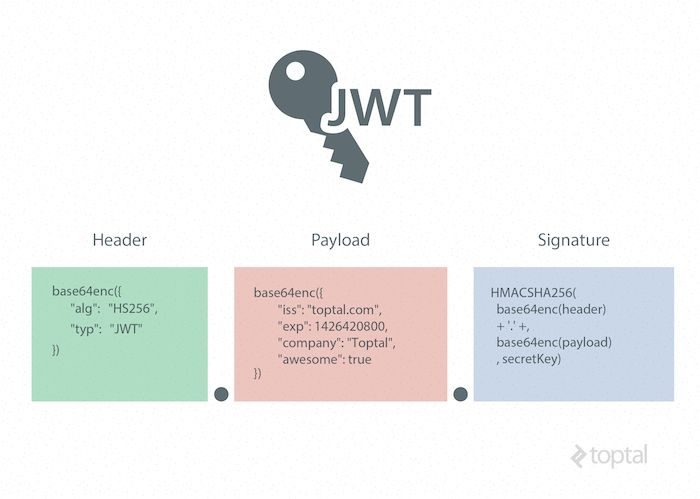
\includegraphics[width=.6\columnwidth]{./img/new/jwt_token.png}%
	\end{center}
	\caption{JWT токен}%
	\label{pic:jwt_token}%
\end{figure}

JWT токен состоит из трех частей, разделенных точками:

\begin{itemize}
    \item \textbf{Header (Заголовок)} - содержит тип токена и алгоритм шифрования. Обычно используется алгоритм HS256.
    \item \textbf{Payload (Полезная нагрузка)} - содержит утверждения (claims) о пользователе, такие как идентификатор, роль, время истечения токена и другие не часто меняющиеся пользовательские данные.
    \item \textbf{Signature (Подпись)} - создается путем шифрования заголовка и полезной нагрузки с использованием секретного ключа. Подпись гарантирует целостность данных и аутентичность токена.
\end{itemize}

Каждая часть токена кодируется в формате Base64. Полученные части соединяются точками, образуя единую строку - JWT токен.


\section{Модель представления узлов и сегментов образований в щитовидной железе}

Интеллектуальная часть ассистента анализирует УЗИ снимки щитовыдной железы на наличие образований как злокачественных, так и доброкачественных. Как правило узи сники представляют собдой кинопетлю щитовидной железы снятой под различными углами. \\
Исходя из этого модель представления описывает физические узлы, снятые под разными углами. Проекции этих узлов, мы будем обозначать контурами.

схема представления:
\begin{figure}[H]%
	\begin{center}
		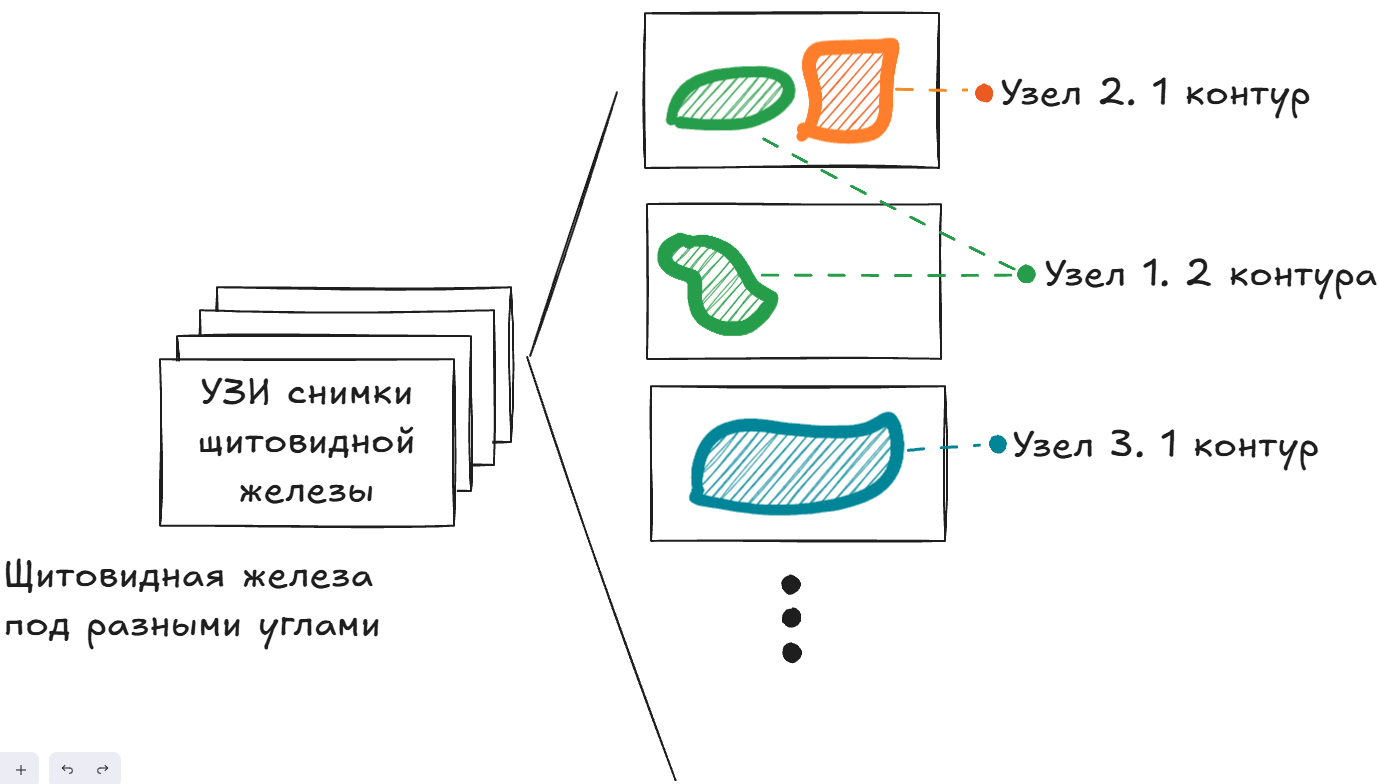
\includegraphics[width=.6\columnwidth]{./img/new/nodes_segments_model.png}%
	\end{center}
	\caption{Модель представления узлов и сегментов}%
	\label{pic:nodes_segments_model}%
\end{figure}

\section{Функциональных требований к системе Интеллектуального ассистента врача щитовидной железы}

Система Интеллектуального ассистента врача щитовидной железы является комплексным сервисом для врача и пациента, позволяющая анализировать УЗИ снимки щитовыдной железы.
Для начала, в системе требуется возможность регистрировать аккаунты врачей и пациентов. Необходима система авторизации и аутентификации пользотелей реализованная по JWT схеме. 
Необходимо хранить информацию о врачах, пациентах и медицинских карточках пациентов.
Для части системы отвечающей за УЗИ следует выдвинуть следующие требования. Система должна загружать снимки УЗИ и сохранять их в хранилище. 
Система должна передавать интеллектуальной части ИИ ассистента снимок УЗИ на обработку. 
Система должна получать результаты обработки от интеллектуальной части ИИ ассистента и сохранять их в базу данных. Результат обработки УЗИ интеллектуальной частью системы, должен
соответствовать модели представления узлов и сегментов.

Таким образом, можно сформировать следующие функциональные требования к системе:
\begin{itemize}
  \item Регистрация врачей и пациентов в системе
  \item Аутентификация и авторизация врачей и пациентов посредством JWT 
  \item Хранение и предоставление информации о врачах, пациентах и медицинских карточках пациентов
  \item Загрузка и хранение УЗИ снимков
  \item Разбиение УЗИ снимков на единичные кадры
  \item Передача УЗИ снимков на обработку интеллектуальной части системы. Сохранение результатов обработки в виде модели узлов и сегментов
\end{itemize}

\subsection{Выявление предметных областей системы}

Исходя из функциональных требований к системе, можно выявить следующие предметные области:\\
\textbf{Авторизация и аутентификация} - область отвечающая за регистрацию и аутентификацию пользователей 
в системе. Вся логика по обработке, хранению и предоставлению JWT также осуществляется в этой области. 
Дальнейшая интеграции с сторонними системами в которых требуется учетные данные пользователей, будут осущетвлять 
посредтсвом ресурсов этой области. \\
\textbf{Управление пользователями} - область отвечающая за хранение и предоставление информации о врачах и пациентах. 
Реализует связь между пациентами и врачами, позволяет создавать историю анализов УЗИ снимков у пациентов, 
смотреть вердиткты ассистента и врача на различные анализы \\
\textbf{Управление УЗИ снимками} - область ответственная за УЗИ снимки: флоу их обработки, хранения результатов обработки, 
предоставление результатов врачам и пациентам. Предоставляет функционал изменения, создания и удаления узлов и сегментов.\\
\textbf{Интеллектуальная часть} - область отвечающая за обработку УЗИ снимков, классификацию узлов и сегментов.

\section{Моделирование системы}

\subsection{Компонент авторизации и аутентификации}

Функциональные требования к компоненту аутентификации:
\begin{itemize}
  \item Хранение базы данных пользователей, паролей, почт и другой чувствительной информации
  \item Шифрование паролей с применением соли и хэша
  \item Возможность регистрировать пользователей, врачей и пациентов
  \item Создание, верификации и подпись JWT ключей для авторизации
  \item Обменивать логин и пароль пользователя на JWT токен
  \item Обновления JWT токена
\end{itemize}

Исходя из функциональных требований, модель базы данных:
\begin{figure}[H]%
	\begin{center}
		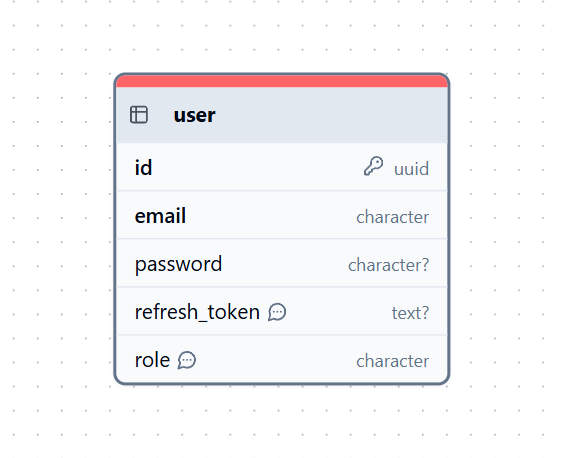
\includegraphics[width=.5\columnwidth]{./img/new/auth_db.png}%
	\end{center}
	\caption{Модель базы данных компонента авторизации и аутентификации}%
	\label{pic:auth_db}%
\end{figure}

Общая модель компонента авторизации и аутентификации:
\begin{figure}[H]%
	\begin{center}
		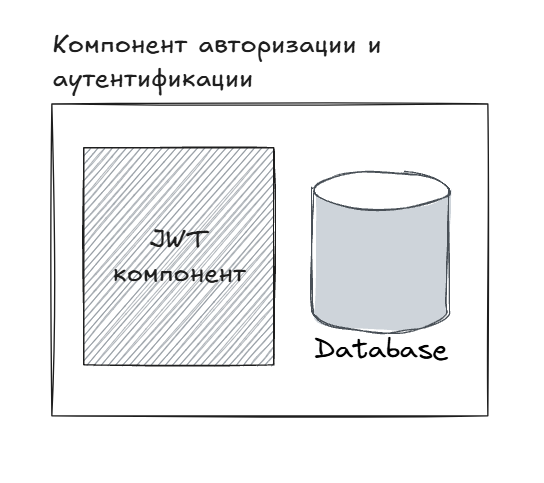
\includegraphics[width=.6\columnwidth]{./img/new/auth_model.png}%
	\end{center}
	\caption{Модель компонента авторизации и аутентификации}%
	\label{pic:auth_model}%
\end{figure}


\subsection{Компонент Управление УЗИ снимками}

Функциональные требования к компоненту Управление УЗИ снимками:
\begin{itemize}
  \item Принимать кинопетлю кадров узи, разбивать и сохранять ее по кадрам.
  \item Передавать интеллектуальной части системы узи, для обработки.
  \item Сохранять результаты обработки узлов и сегментов в базу данных.
  \item Предоставлять возможность просматривать результаты обработки узлов и сегментов.
  \item Предоставлять возможность совершать CRUD операции над узлами, сегментами, узи, ti-rads, images.
\end{itemize}

Тогда для соответствия требованиям, модель базы данных:
\begin{figure}[H]%
	\begin{center}
		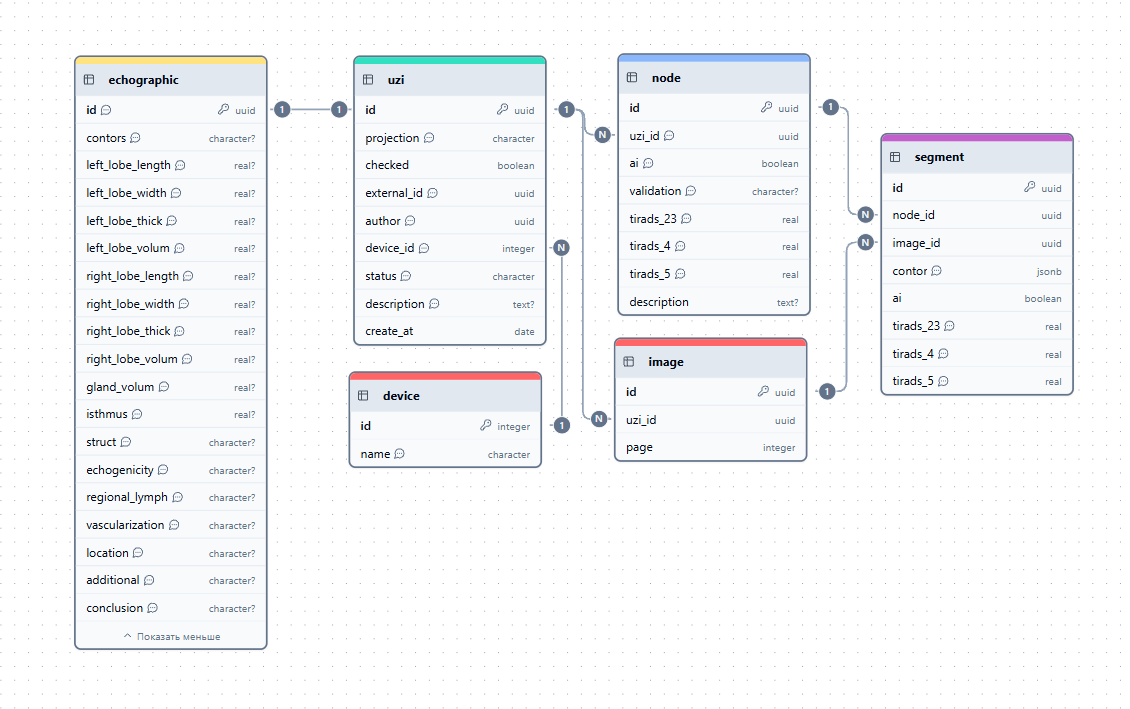
\includegraphics[width=.9\columnwidth]{./img/new/uzi_db.png}%
	\end{center}
	\caption{Модель базы данных компонента Управление УЗИ снимками}%
	\label{pic:uzi_db}%
\end{figure}


Общая модель компонента Управление УЗИ снимками:
\begin{figure}[H]%
	\begin{center}
		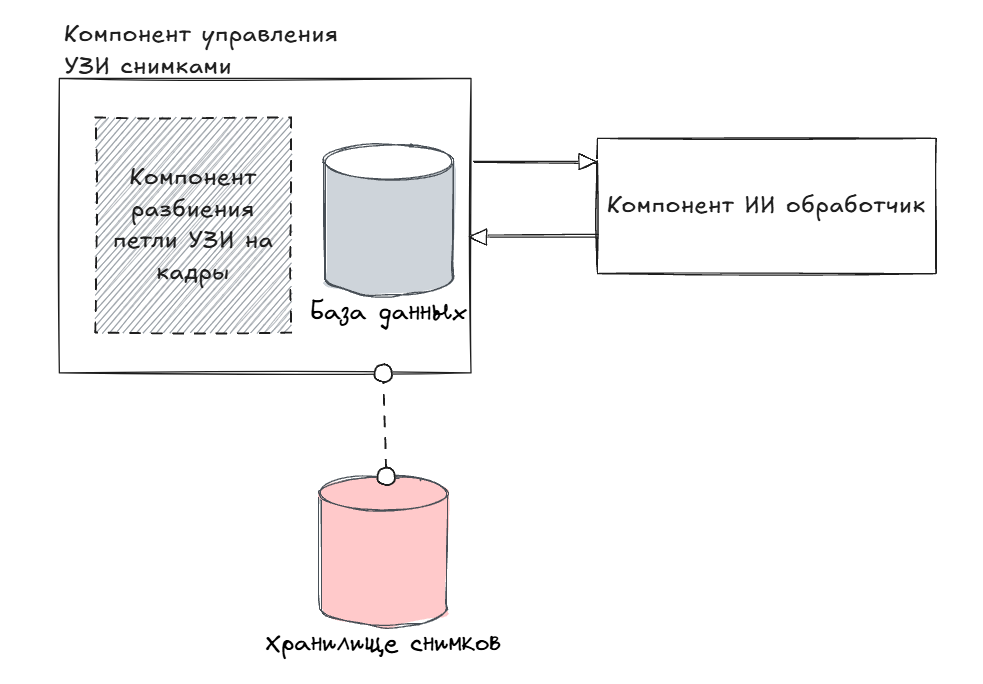
\includegraphics[width=.6\columnwidth]{./img/new/uzi_model.png}%
	\end{center}
	\caption{Модель компонента Управление УЗИ снимками}%
	\label{pic:uzi_model}%
\end{figure}

\subsection{Компонент Управление пользователями}

Функциональные требования к компоненту Управление пользователями:
\begin{itemize}
  \item Хранение публичной информации о врачах и пациентах
  \item Хранить историю болезни пациентов, связанную с УЗИ снимками
  \item Возможность врачам вести историю болезни пациентов, добавлять и удалять пациентов
\end{itemize}

Исходя из функциональных требований, модель базы данных:
\begin{figure}[H]%
	\begin{center}
		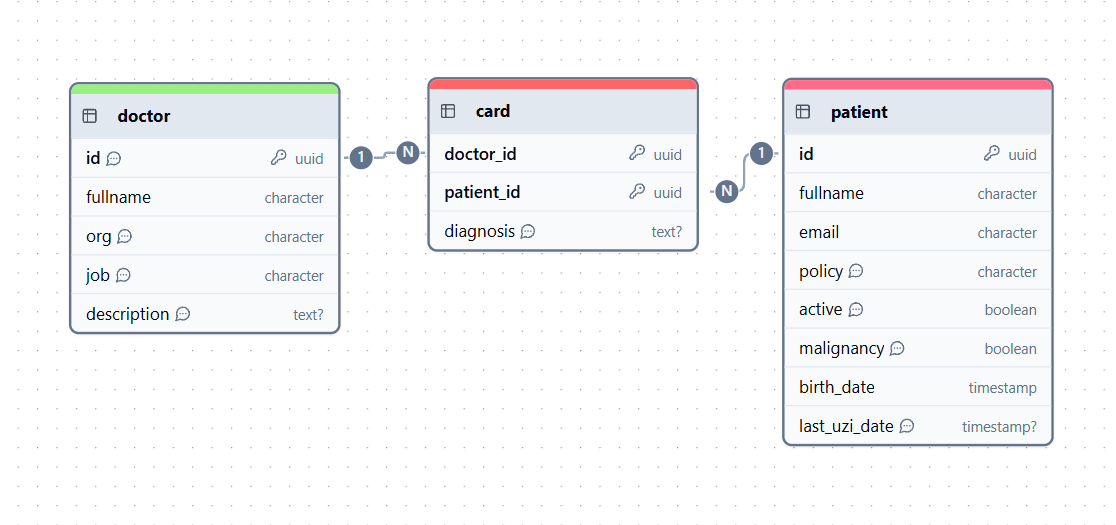
\includegraphics[width=.5\columnwidth]{./img/new/med_db.png}%
	\end{center}
	\caption{Модель базы данных компонента Управление пользователями}%
	\label{pic:med_db}%
\end{figure}

\subsection{Модель системы}

На основе функциональных требований к системе и разделение ее на предметные области, спроектируем модель системы.\\
В соответствии с предметными областями, разобьем систему на модули: модуль аутентификации, модуль управления врачей и пациентов, модуль управления УЗИ снимков, модуль интеллектуальной части.\\

\begin{figure}[H]%
	\begin{center}
		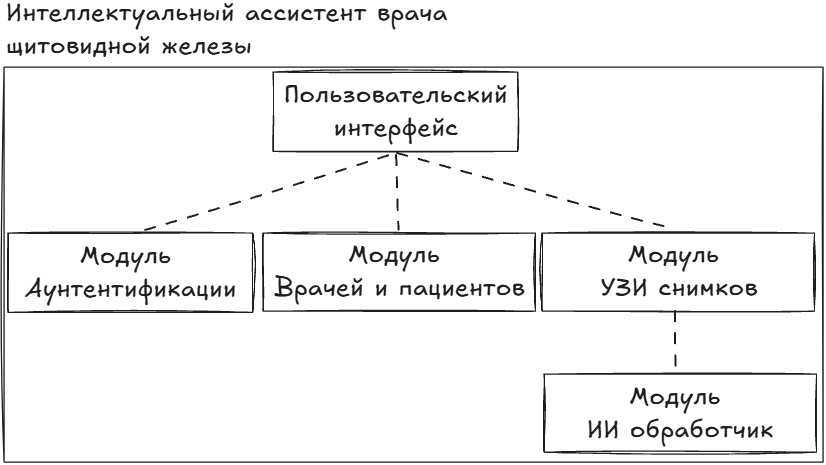
\includegraphics[width=.6\columnwidth]{./img/new/system_model.png}%
	\end{center}
	\caption{Модель системы}%
	\label{pic:system_model}%
\end{figure}

\section{Обощенная модель компонента системы}

Каждый компонент системы проектируется с учетом подхода Clean Architecture, разбиваясь на слои.
Так как система разбита на компоненты по предметным областям, каждый компонент получается достаточно изолированным поэтому не 
требует нарушения принципов разбиения компонента на слои для реализации.
ветствовать приведенной.

Обощенная модель компонента системы будет представлять собой модель типового микросервиса.

\begin{figure}[H]%
	\begin{center}
		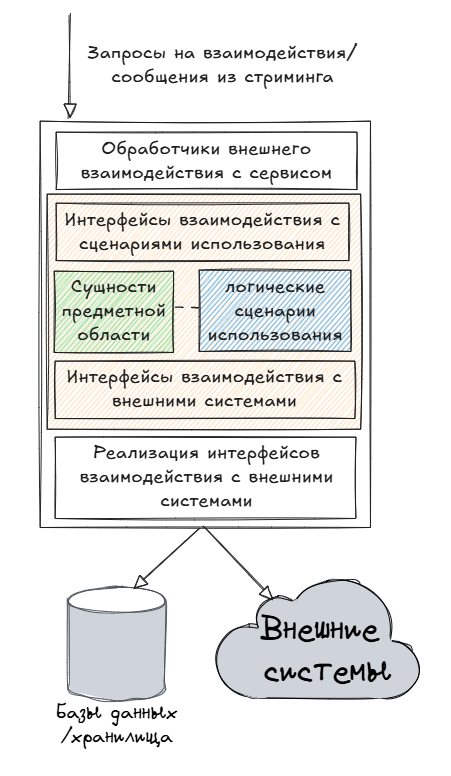
\includegraphics[width=.6\columnwidth]{./img/new/component_model.png}%
	\end{center}
	\caption{Модель компонента системы}%
	\label{pic:component_model}%
\end{figure}

\section{Выводы}

Были спроектированы модели компонентов системы. Объединением всех этих моделей является
модель самой системы. Модели соответствуют и учитывают все функциональные требования к системе, а также к конкретному компоненту.

% В этой главе описываются разработанные/модифицированные модели/методы/
% алгоритмы, или/и описывается применение известных стандартных методов. Также, 
% в конце главы обычно приводится общая архитектура программной системы, 
% вытекающая из описанной теории. Приведенные ниже заголовки подразделов так же 
% весьма примерные и сильно зависят от особенностей конкретной работы.

% Формулы и их части необходимо набирать в математическом режиме
% (символ \verb|$|). Во избежание переноса длинных формул между строками их 
% стоит размещать по центру колонки, например,
% \begin{center}
% $S a b c = (\lambda x y z. x z (y z)) a b c = a c (b c)$,
% \end{center}
% \noindent и, если абзац после формулы продолжается, необходимо использовать 
% \verb|\noindent|.

% Для набора правил вывода можно использовать пакет \texttt{mathpartir.sty}. 
% Правила вывода могут быть вынесены в виде рисунка (см. рис. 
% \ref{img:inferrules}).

% \begin{figure}[t]
%   \centering
%     \begin{mathpar}
%       \inferrule{
%         M \to M'
%       }{
%         N M \to N M'
%       } \quad (\mu) \and 
%       \inferrule{
%         M \to M'
%       }{
%         M N \to M' N
%       } \quad (\nu) \and
%       \inferrule{
%         M \to M'
%       }{
%         \lambda x. M \to \lambda x. M'
%       } \quad (\xi)
%     \end{mathpar}
%   \caption{Правила редукции}
%   \label{img:inferrules}
% \end{figure}

% Для оформления определений, теорем, доказательств и т.~п. могут быть 
% использованы соответствующие окружения, например:

% \begin{definition}
% (высказывание)
% Высказыванием называется любое истинное или ложное утверждение.
% \end{definition}


% \section{Модель системы \dots}

% \dots




% \section{Метод решения задачи для \dots}

% \dots





% \section{Алгоритмы вычисления \dots}

% \dots





% \section{Обобщенная архитектура и интерфейсы \dots}

% В ряде случаев, все или некоторые результаты проектирования могут быть представлены во второй главе. Обычно же архитектура описывается в третьей главе.

% \section{Выводы}

% Необходимо перечислить, какие теоретические результаты были получены с 
% указанием степени новизны. Например: <<Была разработана такая-то модель. Она 
% представляет собой адаптированную версию модели $X$, в которой уравнение $Z$ 
% заменено на уравнение $Z'$>>. Еще пример: <<Была предложена такая-то 
% архитектура, она отличается от типовой в том-то и том-то. Это позволяет 
% избежать таких-то проблем.>>. При этом не следует заниматься <<высасыванием из 
% пальца>>: <<Поставленная задача является типовой; для ее решения применены 
% стандартные средства (перечислить, какие).>>.

%%% Local Variables:
%%% TeX-engine: xetex
%%% eval: (setq-local TeX-master (concat "../" (seq-find (-cut string-match ".*-3-pz\.tex$" <>) (directory-files ".."))))
%%% End:
